% Este trabalho está licenciado sob a Licença Atribuição-CompartilhaIgual 4.0 Internacional Creative Commons. Para visualizar uma cópia desta licença, visite http://creativecommons.org/licenses/by-sa/4.0/deed.pt_BR ou mande uma carta para Creative Commons, PO Box 1866, Mountain View, CA 94042, USA.

\chapter{Linguagem de Programação}\label{cap_lingua}
\thispagestyle{fancy}

\section{Computador}\label{cap_lim_sec_computador}

\begin{flushright}
  [YouTube] | [Vídeo] | [Áudio] | [Contatar]
\end{flushright}

\hl{Um computador\footnote{Consulte \href{https://pt.wikipedia.org/wiki/Computador}{Wikipédia: Computador} para uma introdução sobre a história e outras questões sobre computadores.} é um \emph{sistema computacional} de elementos físicos (\emph{hardware}) e elementos lógicos (\emph{software})}.

\hl{O \emph{hardware} são suas partes mecânicas, elétricas e eletrônicas} como: fonte de energia, teclado, mouse/painel tátil, monitor/tela, dispositivos de armazenagem de dados (HDD, {\it hard disk drive}; SSD, {\it solid-state drive}; RAM, {\it random-access memory}; etc.), dispositivos de processamento (CPU, {\it central processing unit}, GPU, {\it graphics processing unit}), conectores de dispositivos externos (microfone, caixa de som, fone de ouvido, USB, etc.), placa mãe, etc..

\hl{O \emph{software} é toda a informação processada pelo computador}, qualquer código executado e qualquer dado usado nas computações.

\begin{figure}[H]
  \centering
  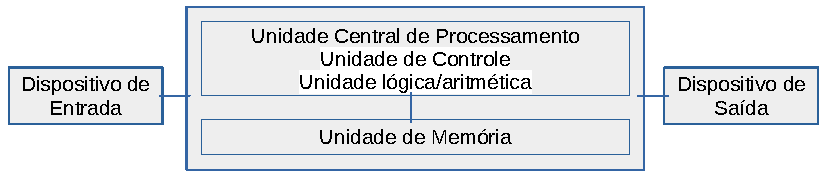
\includegraphics[width=\textwidth]{./cap_lingua/dados/fig_arqVonNeumann/main}
  \caption[Arquitetura de von Neumann]{Arquitetura de computador de von Neumann.}
  \label{cap_lim_sec_computador:fig:arqVonNeumann}
\end{figure}

Os computadores que comumente utilizamos seguem a arquitetura de John von Neumann\footnote{John von Neumann, 1903 - 1957, matemático húngaro, naturalizado estadunidense. Fonte: \href{https://pt.wikipedia.org/wiki/John_von_Neumann}{Wikipédia}.}, que consiste em dispositivo(s) de entrada de dados, unidade(s) de processamento, unidade(s) de memória e dispositivo(s) de saída de dados (Figura~\ref{cap_lim_sec_computador:fig:arqVonNeumann}).

\begin{itemize}
\item \emph{Dispositivos de entrada e saída}

  São elementos do computador que permitem a comunicação humana (usuária(o)) com a máquina.

  \begin{itemize}
  \item \emph{Dispositivos de entrada}

    São elementos que permitem o fluxo de informação da(o) usuária(o) para a máquina. Exemplos são: teclado, mouse/painel tátil, microfone, etc.

  \item \emph{Dispositivos de saída}

    São elementos que permitem o fluxo de informação da máquina para a(o) usuária(o). Exemplos são: monitor/tela, alto-falantes, luzes espia, etc.
  \end{itemize}

\item \emph{Unidade central de processamento}

  A \emph{CPU} (do inglês, {\it Central Processing Unit}) é o elemento de processa as informações e é composta de \emph{unidade de controle}, \emph{unidade lógica e aritmética} e de \emph{memória cache}.

  \begin{itemize}
  \item \emph{Unidade de controle}

    Coordena as execuções do processador: busca e decodifica instruções, lê e escreve no {\it cache} e controla o fluxo de dados.

  \item \emph{Unidade lógica/aritmética}

    Executa as instruções operações lógicas e aritméticas, por exemplo: executar a adição, multiplicação, testar se dois objetos são iguais, etc.

  \item \emph{Memória cache}

    Memória interna da CPU muito mais rápida que as memórias RAM e dispositivos e armazenamento HDD/SSD. É um dispositivo de memória de pequena capacidade e é utilizada como memória de curto prazo e diretamente acessada.
  \end{itemize}

\item \emph{Unidades de memória}

  As unidades de memória são elementos que permitem o armazenamento de dados/objetos. Como memória principal tem-se a \emph{ROM} (do inglês, {\it Read Only Memory}) e a \emph{RAM} (do inglês, {\it Random Access Memory}) e como memória de massa/secundária tem-se HDD, SSD, entre outras.

\item \emph{Memória ROM}

  A memória ROM é utilizada para armazenamento de dados/objetos necessários para dar início ao funcionamento do computador. Por exemplo, é onde a BIOS (dos inglês, {\it Basic Input/Output System}, Sistema Básico de Entrada e Saída) é armazenada. Ao ligarmos o computador este programa é iniciado e é responsável por fazer o gerenciamento inicial dos diversos dispositivos do computador e carregar o \emph{sistema operacional} (conjunto de programas cuja função é de gerenciar os recursos do computador e controlar a execução de programas).

\item \emph{Memória RAM}

  Memória de acesso rápido utilizada para dados/objetos de uso frequente durante a execução de programas. É uma memória volátil, i.e. toda a informação guardada nela é perdida quando o computador é desligado.

\item \emph{Memória de massa/secundária}

  Memória de massa ou secundária são usadas para armazenar dados/objetos por período longo. Normalmente, são dispositivos HDD ou SSD, os dados/objetos são guardados mesmo que o computador seja desligado e contém grande capacidade de armazenagem.   
\end{itemize}

\hl{Os \emph{software} são os elementos lógicos de um sistema computacional, são programas de computadores que contém as instruções que gerenciam o \emph{hardware} para a execução de tarefas específicas}, por exemplo, imprimir um texto, gravar áudio/vídeo, resolver um problema matemático, etc. Programar é o ato de criar programas de computadores.

\subsection{Linguagem de programação}

\hl{As informações fluem no computador codificadas como registros de {\it bits}}\footnote{Usualmente de tamanho $64$-{\it bits}.} (sequência de zeros ou uns). Há registros de instrução e de dados. Programar diretamente por registros é uma tarefa muito difícil, o que levou ao surgimento de linguagens de programação. \hl{Uma \emph{linguagem de programação}\footnote{Código de programação, código de máquina ou linguagem de máquina.} é um método padronizado para escrever instruções para execução de tarefas no computador}. As instruções escritas em uma linguagem são interpretadas e/ou compiladas por um software (interpretador ou compilador) da linguagem que decodifica as instruções em registros de instruções e dados, os quais são efetivamente executados na máquina.

Existem várias linguagens de programação disponíveis e elas são classificadas por diferentes características. Uma \emph{linguagem de baixo nível} (por exemplo, \href{https://pt.wikipedia.org/wiki/Linguagem_assembly}{Assembly}) é aquela que se restringe às instruções executadas diretamente pelo processador, enquanto que uma \emph{linguagem de alto nível} contém instruções mais complexas e abstratas. Estas contém sintaxe mais próxima da linguagem humana natural e permitem a manipulação de objetos mais abstratos. Exemplos de linguagens de alto nível são: \href{https://pt.wikipedia.org/wiki/BASIC}{Basic}, \href{https://pt.wikipedia.org/wiki/Java\_(linguagem\_de\_programa\%C3\%A7\%C3\%A3o)}{Java}, \href{https://pt.wikipedia.org/wiki/JavaScript}{Javascript}, \href{https://pt.wikipedia.org/wiki/MATLAB}{MATLAB}, \href{https://pt.wikipedia.org/wiki/PHP}{PHP}, \href{https://pt.wikipedia.org/wiki/R\_(linguagem_de_programa\%C3\%A7\%C3\%A3o)}{R}, \href{https://pt.wikipedia.org/wiki/C\%2B\%2B}{C/C++}, {\python}, etc.

\hl{Em geral, não existe uma melhor linguagem, cada uma tem suas características que podem ser mais ou menos adequadas conforme o programa que se deseja desenvolver}. Por exemplo, para um site de internet, linguagens como \href{https://pt.wikipedia.org/wiki/JavaScript}{Javascript} e \href{https://pt.wikipedia.org/wiki/PHP}{PHP} são bastante úteis, mas não no desenvolvimento de modelagem matemática e computacional. Nestes casos, \href{https://pt.wikipedia.org/wiki/C\%2B\%2B}{C/C++} é uma linguagem mais apropriada por conter várias estruturas de programação que facilitam a modelagem computacional de problemas científicos. Agora, \href{https://pt.wikipedia.org/wiki/R\_(linguagem_de_programa\%C3\%A7\%C3\%A3o)}{R} é uma linguagem de alto nível com diversos recursos dedicados às áreas de ciências de dados e estatística. Usualmente, utiliza-se mais de uma linguagem no desenvolvimento de programas mais avançados. A ideia é de explorar o melhor de cada linguagem na criação de programas eficientes na resolução dos problemas de interesse.

Nestas notas de aula, \hl{{\python}} é a linguagem escolhida para estudarmos algoritmos e programação. Trata-se de uma \hl{linguagem de alto nível, \emph{interpretada}, \emph{dinâmica} e \emph{mutiparadigma}}. Foi lançada por Guido van Rossum\footnote{Guido van Rossum, 1956-, matemático e programador de computadores holandês. Fonte: \href{https://pt.wikipedia.org/wiki/Guido\_van\_Rossum}{Wikipédia}.} em 1991 e, atualmente, é desenvolvida de forma comunitária, aberta e gerenciada pela ONG \href{https://pt.wikipedia.org/wiki/Python_Software_Foundation}{Python Software Foundation}. A linguagem foi projetada para priorizar a legibilidade do código. Parte da filosofia da linguagem é descrita pelo poema \href{https://pt.wikipedia.org/wiki/Zen_de_Python}{The Zen of Python}. Pode-se lê-lo pelo {\it easter egg} {\python}:
\begin{lstlisting}
  >>> import this
\end{lstlisting}

\begin{itemize}
\item \emph{Linguagem interpretada}

  {\python} é uma linguagem interpretada. Isso significa que o \emph{código-fonte} escrito em linguagem {\python} é interpretado por um programa (interpretador {\python}). Ao executar-se um código, o interpretador lê uma linha do código, decodifica-a como registros para o processador que os executa. Executada uma linha, o interpretador segue para a próxima até o código ter sido completadamente executado.

\item \emph{Linguagem compilada}

  Em uma linguagem compilada, como \href{https://pt.wikipedia.org/wiki/C\%2B\%2B}{C/C++}, há um programa chamado de \emph{compilador} (em inglês, {\it compiler}) e outro de \emph{ligador} (em inglês, {\it linker}). O primeiro, cria um programa-objeto a partir do código e o segundo gerencia sua ligação com eventuais bibliotecas computacionais que ele possa depender. O programa-objeto (também chamado de executável) pode então ser executado pela máquina.
\end{itemize}

Em geral, a execução de um programa compilado é mais rápida que a de um código interpretado. De forma simples, isso se deve ao fato de que nesse a interpretação é feita toda de uma vez e não precisa ser refeita na execução de cada linha de código, como no segundo caso. Por outro lado, a compilação de códigos-fonte grandes pode ser bastante demorada fazendo mais sentido quando ele é compilado uma vez e o programa-objeto executado várias vezes. Além disso, linguagens interpretadas podem usar bibliotecas de programas pré-compiladas. Com isso, pode-se alcançar um bom balanceamento entre tempo de desenvolvimento e de execução do código.

O interpretador {\python} também pode ser usado para compilar o código para um arquivo \emph{bytecode}, este é executado muito mais rápido do que o código-fonte em si, pois as interpretações necessárias já foram feitas. Mais adiante, vamos estudar isso de forma mais detalhada.

\begin{itemize}
\item \emph{Linguagem de tipagem dinâmica}

  {\python} é uma linguagem de tipagem dinâmica. Nela, os dados não precisam ser explicitamente tipificados no código-fonte e o interpretador os tipifica com base em regras da própria linguagem. Ao executar operações com os dados, o interpretador pode alterar seus tipos de forma dinâmica.

\item \emph{Linguagem de tipagem estática}

  \href{https://pt.wikipedia.org/wiki/C\%2B\%2B}{C/C++} é um exemplo de uma linguagem de tipagem estática. Em tais linguagens, os dados devem ser explicitamente tipificados no código-fonte com base nos tipos disponíveis. A retipificação pode ocorrer, mas precisa estar explicitamente definida no código.
\end{itemize}

Existem vários \emph{paradigmas de programação} e a linguagem {\python} é multiparadigma, i.e. permite a utilização de mais de um no código-fonte. Exemplos de paradigmas de programação são: \emph{estruturada}, \emph{orientada a objetos}, \emph{orientada a eventos}, etc.. Na maior parte destas notas de aulas, vamos estudar algoritmos para linguagens de programação estruturada. Mais ao final, vamos introduzir aspectos de linguagens orientada a objetos. Estes são paradigmas de programação fundamentais e suas estruturas são importantes na programação com demais paradigmas disponíveis em programação de computadores.

\subsection{Instalação e execução}

\hl{{\python} é um \emph{software aberto}}\footnote{Consulte a licença de uso em \url{https://docs.python.org/3/license.html}.} e está disponível para vários sistemas operacionais ({\linux}, macOS, Windows, etc.) no seu site oficial
\begin{center}
  \url{https://www.python.org/}
\end{center}
Também, está disponível (gratuitamente) na loja de aplicativos dos sistemas operacionais mais usados. Esta costuma ser a forma mais fácil de instalá-lo na sua máquina, consulte a loja de seus sistema operacional. Ainda, há plataformas e IDEs\footnote{IDE, do inglês, {\it Integrated Development enviroment}, ambiente de desenvolvimento integrado} {\python} disponíveis, consulte, como por exemplo, \href{https://www.anaconda.com/}{Anaconda}.

A execução de um código {\python} pode ser feita de várias formas.

\begin{itemize}
\item \emph{Execução iterativa via terminal}

  Em terminal {\python} pode-se executar instruções/comandos de forma iterativa. Por exemplo:
  \begin{lstlisting}
    >>> print('Olá, mundo!')
    Olá, mundo!
    >>> 
  \end{lstlisting}

  \hl{O símbolo }\lstinline+>>>+\hl{ denota o \emph{prompt de entrada}, onde uma instrução {\python} pode ser digitada}. Após digitar, o comando é executada teclando \lstinline+<ENTER>+. Caso o comando tenha alguma \hl{saída de dados}, como no caso acima, esta aparecerá, por padrão, \hl{no \emph{prompt de saída}}, logo abaixo a linha de comando executada. \hl{Um novo símbolo de prompt de entrada aparece ao término da execução anterior}.

\item \emph{Execução de um {\it script}}

  Para códigos com várias linhas de instruções é mais adequado utilizar um aquivo de {\it script} {\python}. Usando-se um editor de texto ou um IDE ditam-se as linhas de comando em um arquivo \lstinline+.py+. Então, {\it script} pode ser executado em um terminal de seu sistema operacional utilizando-se o interpretador {\python}. Por exemplo, assumindo que o código for salvo do arquivo \lstinline+path_to_arq/arq.py+, pode-se executá-lo em um terminal do sistema com
  \begin{lstlisting}
    $ python3 path_to_arq/arq.py 
  \end{lstlisting}%$
  

  IDEs para {\python} fornecem uma ambiente integrado, contendo um campo para escrita do código e terminal {\python} integrado. Consulte, por exemplo, o IDE {\spyder}:
  \begin{center}
    \url{https://www.spyder-ide.org/}
  \end{center}

\item \emph{Execução em um {\it notebook}}

  {\it Notebooks} {\python} são uma boa alternativa para a execução de códigos em um ambiente colaborativo/educativo. Por exemplo, {\jupyter} é um notebook que roda em navegadores de internet. Sua estrutura e soluções também são encontradas em notebooks online (de uso gratuito limitado) como {\colab} e {\kaggle}.  
\end{itemize}

\subsection{Exercícios}

\begin{exer}
  Verifique qual a versão do sistema operacional que está utilizado em seu computador.
\end{exer}
\begin{resp}
  Dica: Em {\linux}, \lstinline+$ uname --all+ ou \lstinline+$ cat /etc/version+.
\end{resp}

\begin{exer}
  Verifique os seguintes elementos de seu computador:
  \begin{enumerate}[a)]
  \item CPUs
  \item Placa(s) gráfica(s)
  \item Memória RAM
  \item Armazenamento HDD/SSD.
  \end{enumerate}
\end{exer}
\begin{resp}
  Dica: Em {\linux}: \lstinline*$ lshw*%$
\end{resp}

\begin{exer}
  Verifique como entrar na \lstinline+BIOS+ de seu computador. Atenção! Não faça  e salve nenhuma alteração, caso não saiba o que está fazendo. Modificações na \lstinline+BIOS+ podem impedir que seu computador funcione normalmente, inclusive, impedir que você inicialize seu sistema operacional.
\end{exer}
\begin{resp}
  Dica: cada computador tem sua forma de acessar a \lstinline+BIOS+. Verifique o manual ou busque na internet pela marca e modelo de seu computador.
\end{resp}

\begin{exer}
  Instale {\python} no seu computador (caso ainda não tenha feito) e abra um terminal {\python}. Nele, escreva uma linha de comando que imprima no prompt de saída a frase ``Olá, meu Python!''.
\end{exer}
\begin{resp}
\begin{lstlisting}
>>> print('Olá, meu Python!')
Olá, meu Python!
>>> 
\end{lstlisting}
\end{resp}

\begin{exer}
  Instale o {\spyder} no seu computador (caso ainda não tenha feito) e use-o para escrever o seguinte {\it script}
\begin{lstlisting}
import math as m
print(f'Número pi = {m.pi}')
print(f'Número de Euler e = {m.e}')
\end{lstlisting}
  Também, execute o {\it script} diretamente em um terminal de seu sistema operacional.
\end{exer}

\begin{exer}
  Use um {\it notebook} {\python} para escrever e executar o código do exercício anterior.
\end{exer}
\begin{resp}
  Dica: use um notebook online {\colab}, {\kaggle} ou {\jupyter}.
\end{resp}

\section{Algoritmos e Programação}\label{cap_lingua_sec_algoprog}

\hl{\emph{Programar} é criar um programa} (um {\it software}) \hl{para ser executado em computador}. Para isso, escreve-se \hl{um código em uma linguagem computacional} (por exemplo, em {\python}), o qual é interpretado/compilado para gerar o programa final. \hl{Linguagens computacionais são técnicas, utilizam uma sintaxe simples, precisa e sem ambiguidades}. Ou seja, para criarmos um programa com um determinado objetivo, precisamos escrever um código computacional técnico, que siga a sintaxe da linguagem escolhida e sem ambiguidades.

\hl{Um \emph{algoritmo} pode ser definido uma sequencia ordenada e sem ambiguidade de passos para a resolução de um problema}.

\begin{ex}\label{cap_lingua_sec_algoprog:ex:areaTriang}
O cálculo da área de um triângulo de base e altura dadas por ser feito com o seguinte algoritmo:
\begin{enumerate}
\item Informe o valor da base $b$.
\item Informe o valor da altura $h$.
\item $\displaystyle a \leftarrow \frac{b\cdot h}{2}$.
\item Imprima o valor de $a$.
\end{enumerate}

\hl{Algoritmos para a programação são pensados para serem facilmente transformados em códigos computacionais}. Por exemplo, o algoritmo acima pode ser escrito em {\python} como segue:
\begin{lstlisting}
b = float(input('Informe o valor da base.\n'))
h = float(input('Informe o valor da altura.\n'))
# cálculo da área
a = b*h/2
print(f'Área = {a}')
\end{lstlisting}
\end{ex}

Para criar um programa para resolver um dado problema, começamos desenvolvendo um algoritmo para resolvê-lo, este algoritmo é implementado na linguagem computacional escolhida, a qual gera o programa final. Aqui, o passo mais difícil costuma ser o desenvolvimento do algoritmo. Precisamos pensar em como podemos resolver o problema de interesse em uma sequência de passos ordenada e sem ambiguidades para que possamos implementá-los em computador.

\hl{Um algoritmo deve ter as seguintes propriedades}:
\begin{itemize}
\item \hl{Cada passo deve estar bem definido}, i.e. não pode conter ambiguidades.
\item \hl{Cada passo deve contribuir de forma efetiva na solução do problema}.
\item \hl{Deve ter número finito de passos} que podem ser \hl{computados em um tempo finito}.
\end{itemize}

\begin{obs}
  A primeira pessoa a publicar um algoritmo para programação foi Augusta Ada King\footnote{Augusta Ada King, 1815 - 1852, matemática e escritora inglesa. Fonte: \href{https://pt.wikipedia.org/wiki/Ada_Lovelace}{Wikipédia}.}. O algoritmo foi criado para computar os \href{https://pt.wikipedia.org/wiki/N\%C3\%BAmeros\_de\_Bernoulli}{números de Bernoulli}\footnote{Jacob Bernoulli, 1655-1705, matemático suíço. Fonte: \href{https://pt.wikipedia.org/wiki/Jakob_Bernoulli}{Wikipédia}.}.
\end{obs}


\subsection{Fluxograma}

\hl{Fluxograma é uma representação gráfica de um algoritmo}. Entre outras, usam-se as seguintes formas para representar tipos de ações a serem executadas:
\begin{itemize}
\item {\bf Terminal}: início ou final do algoritmo.
  \begin{center}
    
\includegraphics{./cap_lingua/dados/fig_fluxograma/terminal}
  \end{center}  
\item {\bf Linha de fluxo}: direciona para a próxima execução.
  \begin{center}
    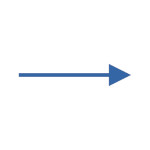
\includegraphics{./cap_lingua/dados/fig_fluxograma/linha}
  \end{center}
\item {\bf Entrada}: leitura de informação/dados.
  \begin{center}
    
\includegraphics{./cap_lingua/dados/fig_fluxograma/entrada}
  \end{center}  
\item {\bf Processo}: ação a ser executada.
  \begin{center}
    
\includegraphics{./cap_lingua/dados/fig_fluxograma/processo}
  \end{center}
\item {\bf Decisão}: ramificação do processamento baseada em uma condição.
  \begin{center}
    
\includegraphics{./cap_lingua/dados/fig_fluxograma/decisao}
  \end{center}
\item {\bf Saída}: impressão de informação/dados.
  \begin{center}
    
\includegraphics{./cap_lingua/dados/fig_fluxograma/saida}
\end{center}
\end{itemize}

\begin{ex}\label{cap_lingua_sec_algoprog:ex:metHeron}
  O \href{https://en.wikipedia.org/wiki/Methods_of_computing_square_roots#Heron's_method}{método de Heron}\footnote{Heron de Alexandria, 10 - 80, matemático e inventor grego. Fonte: \href{https://pt.wikipedia.org/wiki/Heron\_de\_Alexandria}{Wikipédia}.} é um algoritmo para o cálculo aproximado da raiz quadrada de um dado número $x$, i.e. $\sqrt{x}$. Consiste na iteração
  \begin{align}
    s^{(0)} &= \text{approx. inicial},\\
    s^{(i+1)} &= \frac{1}{2}\left(s^{(i)} + \frac{x}{s^{(i)}}\right),
  \end{align}
  para $i=0,1,2,\ldots,n$, onde $n$ é o número de iterações calculadas.

  Na sequência, temos um algoritmo e seus fluxograma e código {\python} para computar a quarta aproximação de $\sqrt{x}$, assumindo $s^{(0)} = x/2$ como aproximação inicial.

  \begin{itemize}
  \item {\bf Algoritmo}
    \begin{enumerate}
    \item Entre o valor de $x$.
    \item Se $x\geq 0$, faça:
      \begin{enumerate}
      \item $s \leftarrow x/2$
      \item Para $i = 0,1,2,3$, faça:
        \begin{enumerate}
        \item $s \leftarrow (s + x/s)/2$.
        \end{enumerate}
      \item Imprime o valor de $s$.
      \end{enumerate}
    \item Senão, faça:
      \begin{enumerate}
      \item Imprime mensagem ``Não existe!''.
      \end{enumerate}
    \end{enumerate}

  \item {\bf Fluxograma}

    \begin{center}
      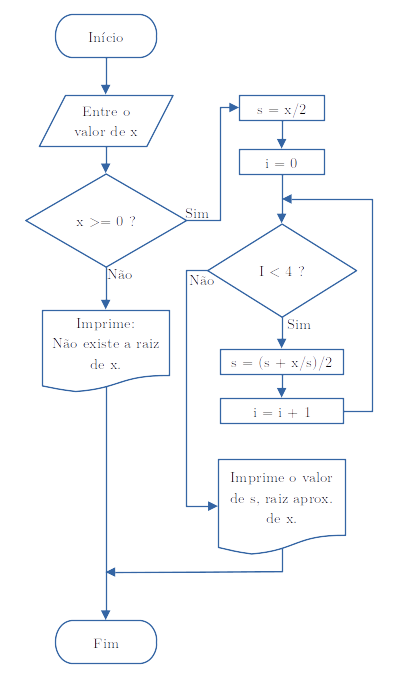
\includegraphics{./cap_lingua/dados/fig_fluxograma/fig}
    \end{center}

  \item {\bf Código {\python}}

\begin{lstlisting}[caption=metHeron.py,label=cap_lingua_sec_algoprog:cod:metHeron]
x = float(input('Entre com o valor de x: '))
if (x >= 0.):
    s = x/2
    for i in range(4):
        s = (s + x/s)/2
    print(f'Raiz aprox. de x = {s}')
else:
    print(f'Não existe!')
\end{lstlisting}
  \end{itemize}

  O algoritmo apresentado acima tem um {\it bug} (um erro)! Consulte o Exercício~\ref{cap_lingua_sec_algoprog:exer:bugHeron}.
\end{ex}

\hl{Algoritmos escritos em uma forma próxima de uma linguagem computacional} são, também, chamados de \hl{\emph{pseudocódigos}}. Na prática, pseudocódigos e fluxogramas são usados para apresentar uma forma mais geral e menos detalhada de um algoritmo. Usualmente, sua forma detalhada é escrita diretamente em uma linguagem computacional escolhida.

\subsection{Exercícios}

\begin{exer}
  Escreva um algoritmo/pseudocódigo e um fluxograma correspondente para o calcular a média aritmética entre dois números $x$ e $y$ dados. Como desafio, tente escrever um código {\python} baseado em seu algoritmo.
\end{exer}

\begin{exer}
  Escreva um algoritmo/pseudocódigo e um fluxograma correspondente para o calcular a área de um quadrado de lado $l$ dado. Como desafio, tente escrever um código {\python} baseado em seu algoritmo.
\end{exer}

\begin{exer}
  Escreva um algoritmo/pseudocódigo e um fluxograma correspondente para o calcular a área de um retângulo de lados $a, b$ dados. Como desafio, tente escrever um código {\python} baseado em seu algoritmo.
\end{exer}

\begin{exer}
  Escreva um algoritmo/pseudocódigo e um fluxograma correspondente para o calcular triângulo retângulo de hipotenusa $h$ e um dos lados $l$ dados. Como desafio, tente escrever um código {\python} baseado em seu algoritmo.
\end{exer}

\begin{exer}
  Escreva um algoritmo/pseudocódigo e um fluxograma correspondente para o calcular o zero de uma função afim
  \begin{equation}
    f(x) = ax + b
  \end{equation}
  dados, os coeficientes $a$ e $b$. Como desafio, tente escrever um código {\python} baseado em seu algoritmo.
\end{exer}

\begin{exer}
  Escreva um algoritmo/pseudocódigo e um fluxograma correspondente para o calcular as raízes reais de um polinômio quadráticos
  \begin{equation}
    p(x) = ax^2 + bx + c
  \end{equation}
  dados, os coeficientes $a$, $b$ e $c$. Como desafio, tente escrever um código {\python} baseado em seu algoritmo.
\end{exer}

\begin{exer}
  A \href{https://pt.wikipedia.org/wiki/S\%C3\%A9rie\_harm\%C3\%B3nica\_(matem\%C3\%A1tica)}{Série Harmônica} é defina por
  \begin{equation}
    \sum_{k=1}^\infty\frac{1}{k} := \frac{1}{1} + \frac{1}{2} + \frac{1}{3} + \cdots
  \end{equation}
  Escreva um algoritmo/pseudocódigo e um fluxograma corresponde para calcular o valor da série harmônica truncada em $k=n$, com $n$ dado. Ou seja, dado $n$, o objetivo é calcular
  \begin{equation}
    \sum_{k=1}^n\frac{1}{k} := \frac{1}{1} + \frac{1}{2} + \cdots + \frac{1}{n}.
  \end{equation}
\end{exer}

\begin{exer}
  O \href{https://pt.wikipedia.org/wiki/E\_(constante\_matem\%C3\%A1tica)}{número de Euler}{\euler} pode ser definido pela série
  \begin{align}
    e &:= \sum_{k=0}^\infty\frac{1}{k!}\\
      &= \frac{1}{0!} + \frac{1}{1!} + \frac{1}{2!} + \frac{1}{3!} + \frac{1}{4!} + \cdots
  \end{align}
  Escreva um algoritmo/pseudocódigo e um fluxograma corresponde para calcular o valor aproximado de $e$ dado pelo truncamento da série em $k=4$, i.e. o objetivo é de calcular
  \begin{align}
    e &\approx \sum_{k=0}^4\frac{1}{k!}\\
      &= \frac{1}{0!} + \frac{1}{1!} + \frac{1}{2!} + \frac{1}{3!} + \frac{1}{4!}\\
      &= \frac{1}{1} + \frac{1}{1} + \frac{1}{1\cdot 2} + \frac{1}{1\cdot 2\cdot 3} + \frac{1}{1\cdot 2\cdot 3\cdot 4}.
  \end{align}
\end{exer}

\begin{exer}\label{cap_lingua_sec_algoprog:exer:bugHeron}
  O algoritmo construído no Exemplo~\ref{cap_lingua_sec_algoprog:ex:metHeron} tem um {\it bug} (um erro). Identifique o {\it bug} e proponha uma nova versão para corrigir o problema. Então, apresente o fluxograma da nova versão do algoritmos. Como desafio, busque implementá-lo em {\python}. 
\end{exer}
\begin{resp}
  Dica: o {\it bug} ocorre quando $x = 0$.
\end{resp}

\section{Dados}\label{cap_lingua_sec_dados}

Informação é resultante do processamento, manipulação e organização de \emph{dados} (altura, quantidade, volume, intensidade, densidade, etc.). \hl{Programas de computadores processam, manipulam e organizam \emph{dados computacionais}}. Os dados computacionais são representações em máquina de dados ``reais''. De certa forma, todo dado é uma abstração e, para ser utilizado em um programa de computador, precisa ser representado em máquina.

Cada dado manipulado em um programa é identificado por um \emph{nome}, chamado de \emph{identificador}. Podem ser variáveis, constantes, funções/métodos, entre outros.
\begin{itemize}
\item \emph{Variável}

  Objetos de um programa que armazenam dados que podem mudar de valor durante a sua execução.

\item \emph{Constantes}

  Objetos de um programa que não mudam de valor durante a sua execução.

\item \emph{Funções e métodos}

  Subprogramas definidos e executados em um programa.
\end{itemize}

\subsection{Identificadores}

\hl{Um identificador é um nome atribuído para a identificação inequívoca de dados que são manipulados em um programa}.

\begin{ex}\label{cap_lingua_sec_dados:ex:reta}
  Vamos desenvolver um programa que computa o ponto de interseção da reta de equação
  \begin{equation}
    y = ax + b
  \end{equation}
  com o eixo $x$ (consulte a Figura~\ref{cap_lingua_sec_dados:fig:ex_reta}).

  \begin{figure}[H]
    \centering
    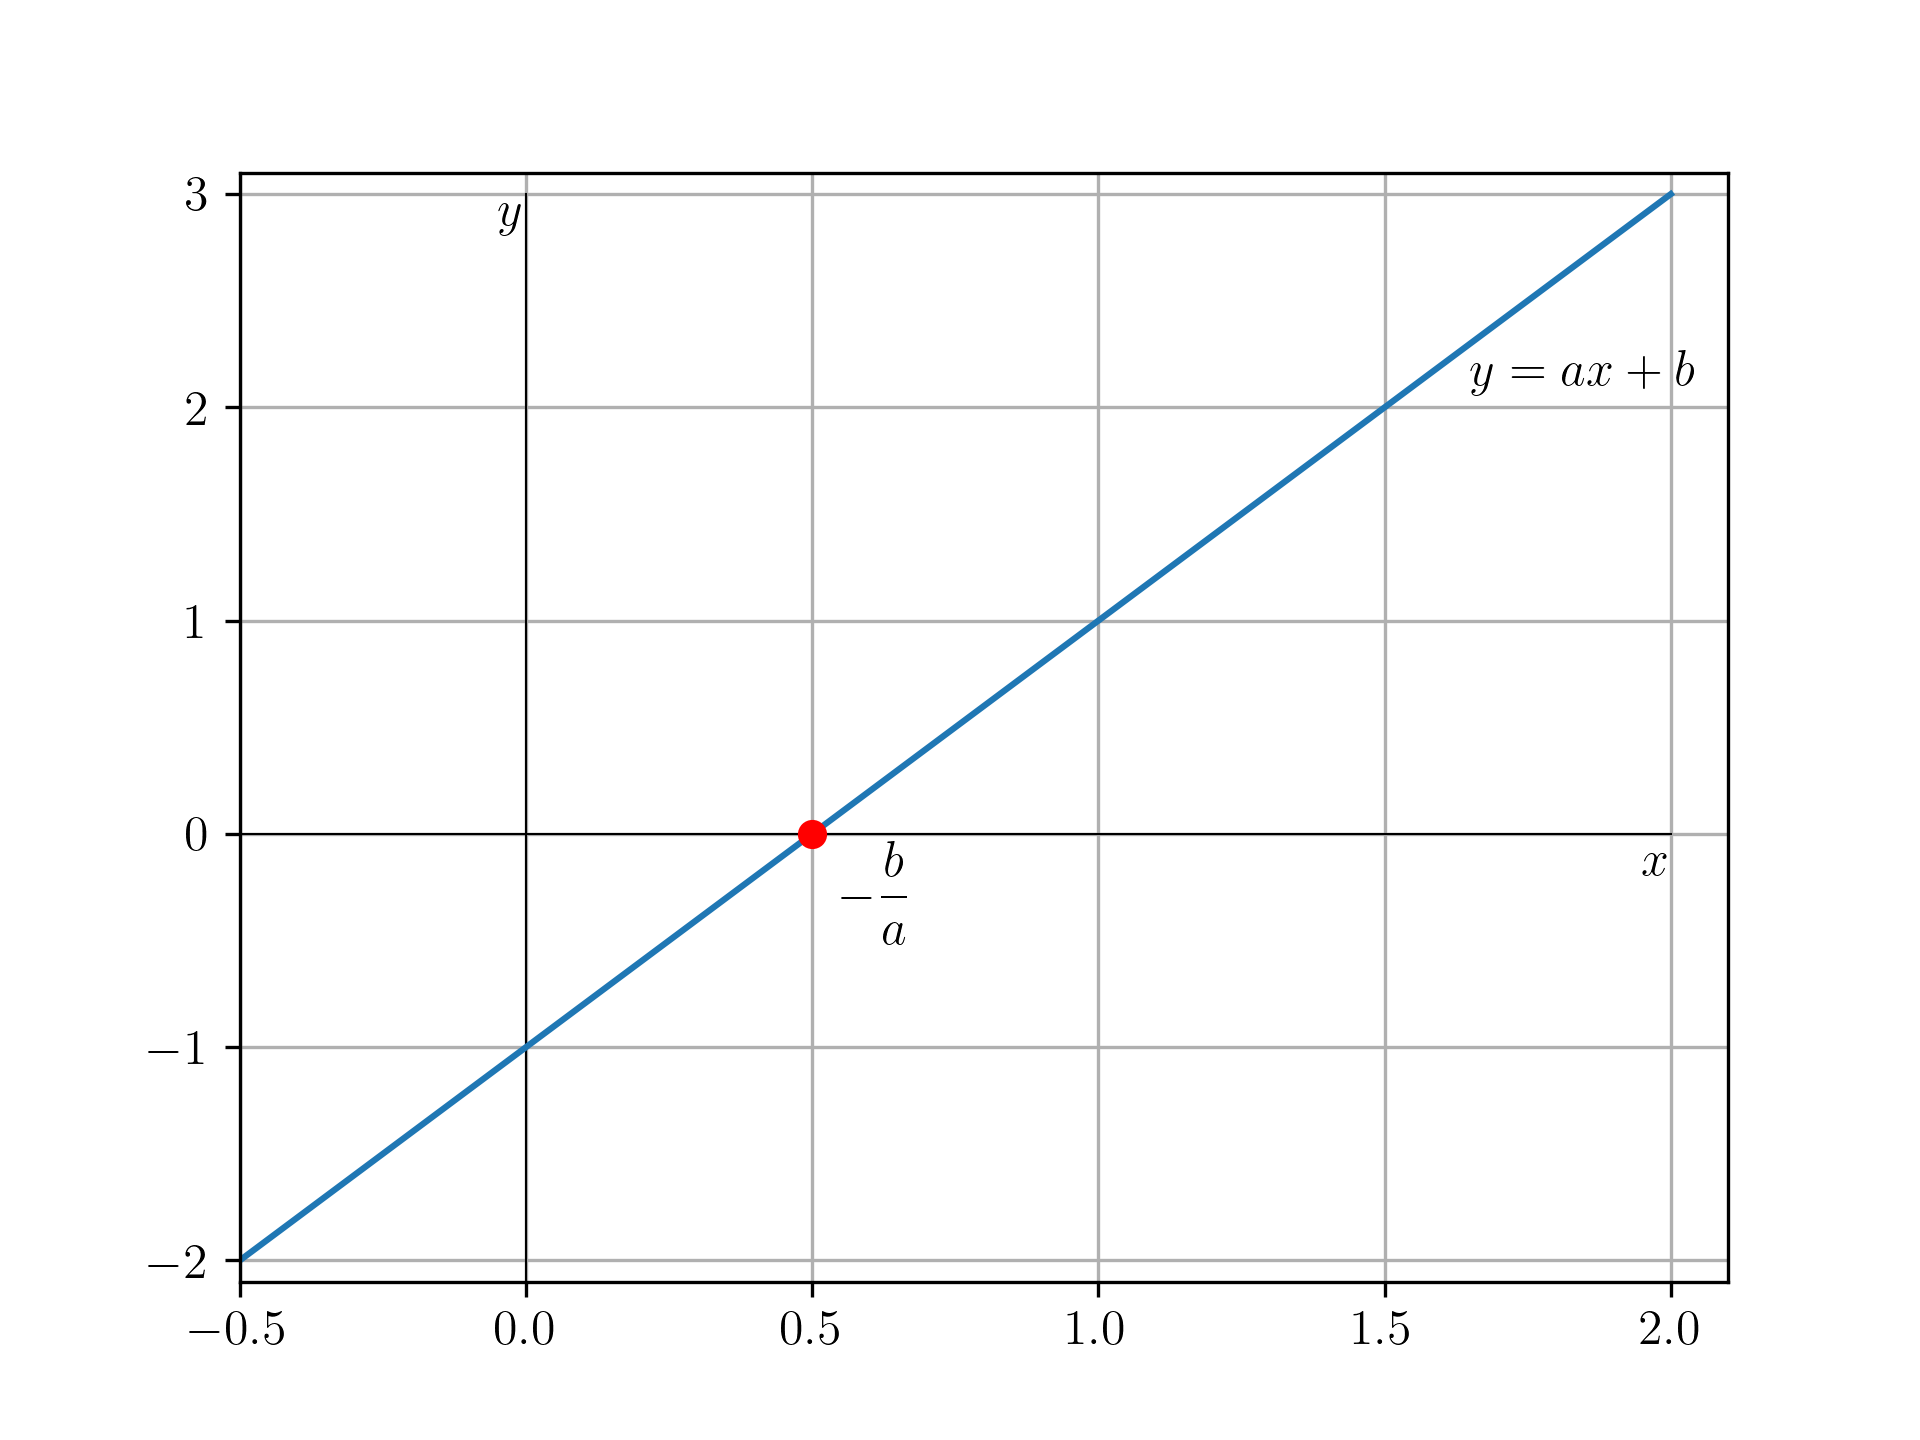
\includegraphics[width=\textwidth]{./cap_lingua/dados/fig_ex_reta/fig}
    \caption{Esboço da reta de equação $y = ax + b$, com $a=2$ e $b=-1$.}
    \label{cap_lingua_sec_dados:fig:ex_reta}
  \end{figure}

  O ponto $x$ em que a reta intercepta o eixo das abscissas é
  \begin{equation}
    x = -\frac{b}{a}
  \end{equation}
  Assumindo que $a=2$ e $b=-1$, segue um algoritmo para a computação.
  \begin{enumerate}
  \item Atribui o valor do \emph{coeficiente angular}:
    \begin{equation}
      a\leftarrow 2.
    \end{equation}
  \item Atribui o valor do \emph{coeficiente linear}:
    \begin{equation}
      b\leftarrow -1.
    \end{equation}
  \item Computa e armazena o valor do \emph{ponto de interseção com o eixo $x$}:
    \begin{equation}
      x \leftarrow -\frac{b}{a}.
    \end{equation}
  \item Imprime o valor de $x$.
  \end{enumerate}

  No algoritmo acima, os identificados utilizados foram: $a$ para o \emph{coeficiente angular}, $b$ para o \emph{coeficiente linear} e $x$ para o \emph{ponto de interseção com o eixo x}.
\end{ex}


\hl{Em {\python}, os identificadores são sensíveis a letras maiúsculas e minúsculas (em inglês, \textit{case sensitive})}, i.e. o identificador \lstinline+nome+ é diferente dos \lstinline+Nome+, \lstinline+NoMe+ e \lstinline+NOME+. Por exemplo:
\begin{lstlisting}
>>> a = 7
>>> print(A)
Traceback (most recent call last):
  File "<stdin>", line 1, in <module>
NameError: name 'A' is not defined. Did you mean: 'a'?
\end{lstlisting}

\hl{Para melhorar a legibilidade de seus códigos, recomenda-se utilizar identificadores com nomes compostos} que ajudem a lembrar o significado do dado a que se referem. No exemplo acima (Exemplo~\ref{cap_lingua_sec_dados:ex:reta}), $a$ representa o \emph{coeficiente angular} da reta e um identificar apropriado seria \lstinline+coefAngular+ ou \lstinline+coef_angular+.

\hl{Identificadores não podem conter caracteres especiais} (\lstinline+*+, \lstinline+&+, \lstinline+%+,
\lstinline+ç+, acentuações, etc.), \hl{espaços em branco} e começar com número. As seguintes convenções para identificadores com nomes compostos são recomendadas:
\begin{itemize}
\item \emph{lowerCamelCase}: \lstinline+nomeComposto+
\item \emph{UpperCamelCase}: \lstinline+NomeComposto+
\item \emph{snake}: \lstinline+nome_composto+
\end{itemize}

Alguns identificadores são palavras reservadas pela linguagem, pois representam dados pré-definidos nela. Veja a lista de identificadores reservados em \href{https://docs.python.org/3/reference/lexical_analysis.html#keywords}{Python Docs: Lexical Analysis: Keywords}.

\begin{ex}
  O algoritmo construído no Exemplo~\ref{cap_lingua_sec_dados:ex:reta} pode ser implementado como segue:
\begin{lstlisting}
coefAngular = 2
coefLinear = -1
intercepEixoX = -coefLinear/coefAngular
print(intercepEixoX)
\end{lstlisting}
\end{ex}

\subsection{Alocação de dados}

Como estudamos acima, \hl{alocamos e referenciamos dados na memória do computador usando identificadores}. Em {\python}, ao executarmos a instrução
\begin{lstlisting}
>>> x = 1
\end{lstlisting}
estamos criando um \emph{objeto} na memória com valor $1$ e \lstinline+x+ é uma referência para este dado alocado na memória. Pode-se imaginar a memória computacional como um sequência de caixinhas, de forma que \lstinline+x+ será a identificação da caixinha onde o valor $1$ foi alocado.

\begin{center}
  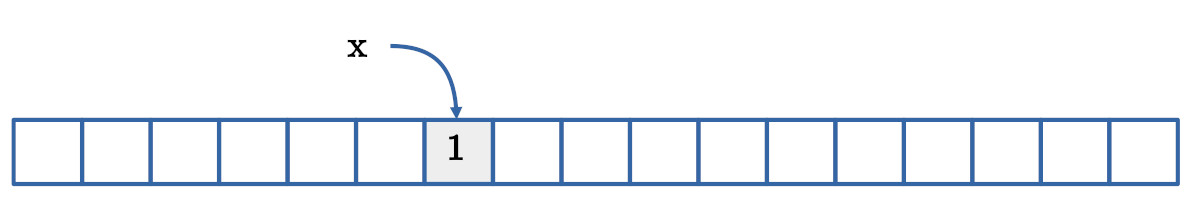
\includegraphics[width=\textwidth]{./cap_lingua/dados/fig_aloc_mem/xRecebe1}
\end{center}

Agora, quando executamos a instrução
\begin{lstlisting}
>>> y = x 
\end{lstlisting}
o identificador \lstinline+y+ passa a referenciar o mesmo local de memória de \lstinline+x+.

\begin{center}
  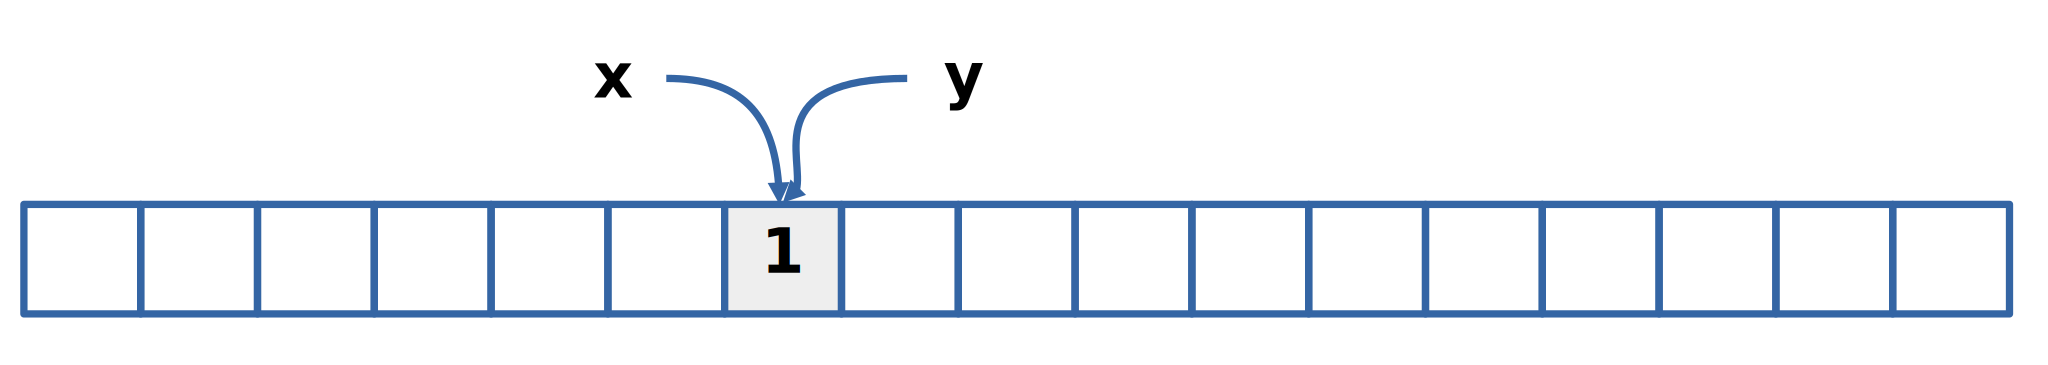
\includegraphics[width=\textwidth]{./cap_lingua/dados/fig_aloc_mem/yRecebex}
\end{center}

Na sequência, se atribuirmos um novo valor para \lstinline+x+
\begin{lstlisting}
>>> x = 2
\end{lstlisting}
este será alocado em um novo local na memória e \lstinline+x+ passa a referenciar este novo local.

\begin{center}
  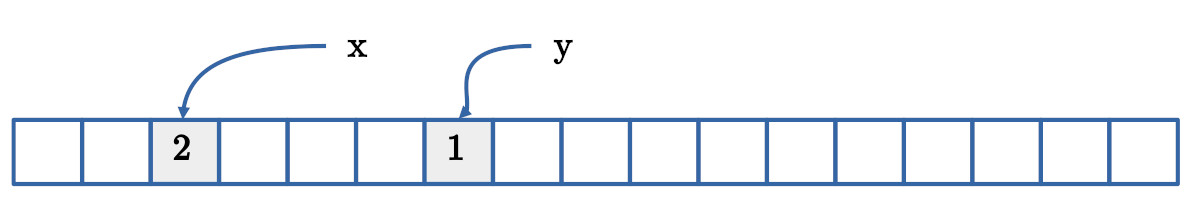
\includegraphics[width=\textwidth]{./cap_lingua/dados/fig_aloc_mem/xRecebe2}
\end{center}

Ainda, se atribuirmos um novo valor para \lstinline+y+
\begin{lstlisting}
>>> y = 3
\end{lstlisting}
este será alocado em um novo local na memória e \lstinline+y+ passa a referenciar este novo local. O local de memória antigo, em que o valor $2$ está alocado, passa a ficar novamente disponível para o sistema operacional.

\begin{center}
  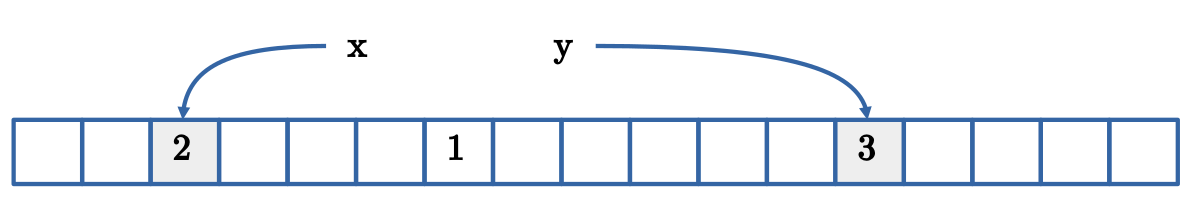
\includegraphics[width=\textwidth]{./cap_lingua/dados/fig_aloc_mem/yRecebe3}
\end{center}

\begin{obs}
  O método {\python} \href{https://docs.python.org/3/library/functions.html?highlight=id#id}{\lstinline+id+} retorna a identidade (endereço da caixinha) de um objeto. Essa identidade deve ser única e constante para cada objeto.
\begin{lstlisting}
>>> x = 1
>>> id(x)
139779845161200
>>> y = x
>>> id(y)
139779845161200
>>> x = 2
>>> id(x)
139779845161232
>>> id(y)
139779845161200
>>> y = 3
>>> id(y)
139779845161264
\end{lstlisting}
\end{obs}

\begin{ex}\normalfont{(\hl{Troca de Variáveis/Identificadores}.)}\label{cap_lingua_sec_dados:ex:trocaVar}
Em várias situações, faz-se necessário permutar dados entre dois identificadores. Sejam
\begin{lstlisting}
x = 1
y = 2
\end{lstlisting}
Agora, queremos permutar os dados, ou seja, queremos que \lstinline+y+ tenha o valor $1$ e \lstinline+x+ o valor $2$. Podemos fazer isso utilizando uma variável auxiliar (em inglês, {\it buffer}).
\begin{lstlisting}
z = x
x = y
y = z
\end{lstlisting}
Verifique!
\end{ex}

\subsection{Exercícios}

\begin{exer}
  Proponha identificadores adequados à linguagem {\python} baseados nos seguintes nomes:
  \begin{enumerate}[a)]
  \item Área
  \item Perímetro do quadrado
  \item Cateto+Cateto
  \item Número de elementos do conjunto A
  \item 77 lados
  \item $f(x)$
  \item $x^2$
  \item $13x$
  \end{enumerate}
\end{exer}
\begin{resp}
  a) \lstinline+area+; b) \lstinline+perimetroQuad+; c) \lstinline+somaCatetos+; d) \lstinline+numElemA+; e) \lstinline+lados77+; f) \lstinline+fx+; g) \lstinline+x2+; h) \lstinline+xv13+
\end{resp}

\begin{exer}
  No Exemplo~\ref{cap_lingua_sec_algoprog:ex:areaTriang}, apresentamos um código {\python} para o cálculo da área de um triângulo. Reescreva o código trocando seus identificadores por nomes mais adequados.
\end{exer}
\begin{resp}
\begin{lstlisting}
base = float(input('Informe o valor da base.\n'))
altura = float(input('Informe o valor da altura.\n'))
# cálculo da área
area = base * altura /2
print(f'Área = {area}')
\end{lstlisting}
\end{resp}

\begin{exer}
  O seguinte código {\python} tem um erro:
\begin{lstlisting}
x = 1
y = X + 1
\end{lstlisting}
  Identifique-o e apresente uma nova versão código corrigido.
\end{exer}
\begin{resp}
  Erro: variável $X$ não foi definida.
\begin{lstlisting}
x = 1
y = x + 1
\end{lstlisting}
\end{resp}

\begin{exer}
  Faça uma representação gráfica da alocação de memória que ocorre para cada uma das instruções {\python} do Exemplo~\ref{cap_lingua_sec_dados:ex:trocaVar} na troca de variáveis. Ou seja, para a seguinte sequência de instruções:
\begin{lstlisting}
x = 1
y = 2
z = x
x = y
y = z
\end{lstlisting}
\end{exer}

\begin{exer}
  No Exemplo~\ref{cap_lingua_sec_dados:ex:trocaVar} fazemos a permutação entre as variáveis \lstinline+x+ e \lstinline+y+ usando um {\it buffer} \lstinline+z+ para guardar o valor de \lstinline+x+. Se, ao contrário, usarmos o {\it buffer} para guardar o valor de \lstinline+y+, como fica o código de permutação entre as variáveis?
\end{exer}
\begin{resp}
  \begin{lstlisting}
    x = 1
    y = 2
    z = y
    y = x
    x = z
    print(x, y)
    2 1
  \end{lstlisting}
\end{resp}

\section{Dados Numéricos e Operações}\label{cap_lingua_sec_numop}

Números são tipos de dados comumente manipulados \hl{em programas de computador}. \hl{Números inteiros e não inteiros são tratados de forma diferente}. Mas, antes de discorrermos sobre essas diferenças, vamos estudar operadores numéricos básicos.

\subsubsection{Operações Numéricas Básicas}

As seguintes operações numéricas estão disponíveis na linguagem {\python}:
\begin{itemize}
\item \lstinline*+*\textbf{: adição}
\begin{lstlisting}
>>> 1 + 2
3
\end{lstlisting}
\item \lstinline+-+\textbf{: subtração}
\begin{lstlisting}
>>> 1 - 2
-1
\end{lstlisting}
\item \lstinline+*+\textbf{: multiplicação}
\begin{lstlisting}
>>> 2*3
6
\end{lstlisting}
\item \lstinline+/+\textbf{: divisão}
\begin{lstlisting}
>>> 5/2
2.5
\end{lstlisting}
\item \lstinline+//+\textbf{: divisão inteira}
\begin{lstlisting}
>>> 5//2
2
\end{lstlisting}
\item \lstinline+%+\textbf{: resto da divisão}
\begin{lstlisting}
>>> 5 % 2
1
\end{lstlisting}
\end{itemize}

A precedência das operações deve ser observada em {\python}. \hl{Uma expressão é executada da esquerda para a direita, mas os operadores tem a seguinte precedência}\footnote{Consulte a lista completa de operadores e suas precedências em \href{https://docs.python.org/3/reference/expressions.html\#operator-precedence}{Python Docs: Expressions: Operator precedence}.}:
\begin{enumerate}
\item \lstinline*-x*\textbf{: oposto de $x$}
\item \lstinline+**+
\item \lstinline+*, /, //, %+
\item \lstinline*+, -*
\end{enumerate}
\hl{Utilizamos parênteses para impor uma precedência diferente}, i.e. expressões entre parênteses \lstinline+()+ são executadas antes das demais.

\begin{ex}
  Estudamos a seguinte computação:
\begin{lstlisting}
>>> 2+8*3/2**2-1
7.0
\end{lstlisting}

  Uma pessoa desavisada poderia pensar que o resultado está errado, pois
  \begin{gather}
    2+8 = 10,\\
    10 \cdot 3 = 30,\\
    30 \div 2 = 15,\\
    15^2 = 225,\\
    225 - 1 = 224.
  \end{gather}
  Ou seja, o resultado não deveria ser $224$? Não, em {\python}, a operação de potenciação \lstinline+**+ tem a maior precedência, depois vem as de multiplicação \lstinline+*+ e divisão \lstinline+/+ (com a mesma precedência, sendo que a mais a esquerda é executada primeiro) e, por fim, vem as de adição \lstinline*+* e subtração \lstinline+-+ (também com a mesma precedência entre si). Ou seja, a instrução acima é computada na seguinte ordem:
  \begin{gather}
    2^2 = 4,\\
    8\cdot 3 = 24,\\
    24\div 4 = 6,\\
    2 + 6 = 8,\\
    8 - 1 = 7.
  \end{gather}

  Para impormos um ordem diferente de precedência, usamos parêntese. No caso acima, escrevemos
\begin{lstlisting}
>>> ((2 + 8)*3/2)**2 - 1
224.0
\end{lstlisting}
\end{ex}

O uso de espaços entre os operandos,em geral, é arbitrário, mas conforme utilizados podem dificultar a legibilidade do código.

\begin{ex}
  Consideramos a seguinte expressão
\begin{lstlisting}
>>> 2 *- 3 + 2
-4
\end{lstlisting}
  Essa expressão é computada na seguinte ordem:
  \begin{gather}
    -~3 = -3\\
    2\cdot(-3) = -6\\
    -6 + 2 = -4
  \end{gather}
  Observamos que ela seria melhor escrita da seguinte forma:
\begin{lstlisting}
>>> 2*-3 + 2
-4
\end{lstlisting}
\end{ex}

\subsection{Números Inteiros}

\hl{Em {\python}, números inteiros são alocados por registros com um número arbitrário de {\it bits}}. Com isso, os maior e menor números inteiros que podem ser alocados dependem da capacidade de memória da máquina. \hl{Quanto maior ou menor o número inteiro, mais {\it bits} são necessários para alocá-lo}.

\begin{ex}
  O método {\python} \href{https://docs.python.org/3/library/sys.html#sys.getsizeof}{\lstinline+sys.getsizeof()+} retorna o tamanho de um objeto medido em {\it bytes} \hl{($1~\textit{byte} = 8~\textit{bits}$)}.
\begin{lstlisting}
>>> import sys
>>> sys.getsizeof(0)
24
>>> sys.getsizeof(1)
28
>>> sys.getsizeof(100)
28
>>> sys.getsizeof(10**9)
28
>>> sys.getsizeof(10**100)
32
>>> sys.getsizeof(10**100) #googol
72
\end{lstlisting}

  O número \href{https://en.wikipedia.org/wiki/Googol}{googol} $10^{100}$ é um número grande\footnote{Por exemplo, o número total de partículas elementares em todo o universo observável é estimado em $10^80$. Fonte: \href{https://en.wikipedia.org/wiki/Eddington_number}{Wikipédia: Eddington number}.}, mas $72$~\textit{bytes} não necessariamente. Um computador com $4$~Gbytes\footnote{$1~\textit{Gbytes} = 1024~\textit{Mbytes}$, $1~\textit{Mbytes} = 1024~\textit{Kbytes}$, $1~\textit{Kbytes} = 1024~\textit{bytes}$.} livres de memória, poderia armazenar um número inteiro que requer um registro de até $4,3\times 10^9~\textit{bytes}$.
\end{ex}

\begin{obs}
  O método {\python} \href{https://docs.python.org/3/glossary.html#term-type}{type()} retorna o tipo de objeto alocado. Números inteiros são objetos da classe \lstinline+int+.
\begin{lstlisting}
>>> type(10)
<class 'int'>
\end{lstlisting}
\end{obs}

\subsection{Ponto Flutuantes}

No {\python}, \hl{números decimais são alocados} pelo padrão \href{https://en.wikipedia.org/wiki/IEEE\_754}{IEEE 774} de aritmética \hl{em ponto flutuante}. Em geral, são usados $64~\textit{bits} = 8~\textit{bytes}$ para alocar um número decimal. Um ponto flutuante tem a forma
\begin{equation}
  x = \pm m\cdot 2^{c-1023},
\end{equation}
onde $m$ é chamada de mantissa (e é um número no intervalo $[1,2)$) e $c\in [0, 2047]$ é um número inteiro chamado de característica do ponto flutuante. A mantissa usa $53~\textit{bits}$, a característica $11~\text{bits}$ e $1~\textit{bit}$ é usado para o sinal do número.

\begin{lstlisting}
>>> import sys
>>> sys.float_info
sys.float_info(max=1.7976931348623157e+308, 
               max_exp=1024, 
               max_10_exp=308, 
               min=2.2250738585072014e-308, 
               min_exp=-1021, 
               min_10_exp=-307, 
               dig=15, 
               mant_dig=53, 
               epsilon=2.220446049250313e-16, 
               radix=2, 
               rounds=1)
\end{lstlisting}

Vamos denotar \lstinline+fl(x)+ o número em ponto flutuante mais próximo do número decimal \lstinline+x+ dado. Quando digitamos
\begin{lstlisting}
>>> x = 0.1
\end{lstlisting}
\hl{O valor alocado na memória da máquina} não \hl{é} \lstinline+0.1+, mas, sim, o \hl{{\lstinline+fl(x)+}}. Normalmente, o \hl{\textbf{épsilon de máquina} $\varepsilon = 2,22\times 10^{-16}$ é uma boa aproximação para o erro (de arredondamento)} entre \lstinline+x+ e \lstinline+fl(x)+.

\subsubsection{Notação Científica}

A \hl{\emph{notação científica}} é a representação de um dado número na forma
\begin{equation}
  d_{n}\ldots d_2d_1d_0,d_{-1}d_{-2}d_{-3}\ldots \times 10^{E},
\end{equation}
onde $d_i$, $i=n, \ldots, 1, 0, -1, \ldots$, são algarismos da base 10. A parte à esquerda do sinal $\times$ é chamada de mantissa do número e $E$ é chamado de expoente (ou ordem de grandeza).

\begin{ex}\label{cap_lingua_sec_numop:ex:notacao_cientifica}
  O número $31,515$ pode ser representado em notação científica das seguintes formas
  \begin{align}
    31,415\times 10^0 &= 3,1415\times 10^{1} \\
                      &= 314,15\times 10^{-1} \\
                      &= 0,031415\times 10^{3},
  \end{align}
  entre outras tantas possibilidades.

  \hl{Em {\python}, usa-se a letra {\lstinline+e+} para separar a mantissa do expoente na notação científica}. Por exemplo
  \begin{lstlisting}
    >>> # 31.415 X 10^0
    >>> 31.415e0
    31.515
    >>> # 3.1415 X 10^1
    >>> 3.1415e1
    31.515
    >>> # 314.15 X 10^-1
    >>> 314.15e-1
    31.515
    >>> # 0.031415 X 10^3
    >>> 0.031415e3
    31.415
  \end{lstlisting}
\end{ex}

No exemplo anterior (Exemplo~\ref{cap_lingua_sec_numop:ex:notacao_cientifica}), podemos observar que a representação em notação científica de um dado número não é única. Para contornar isto, introduzimos a \hl{\emph{notação científica normalizada}}, a qual tem a forma
\begin{equation}
  d_0,d_{-1}d_{-2}d_{-3}\ldots\times 10^{E},
\end{equation}
com $d_0 \neq 0$\footnote{No caso do número zero, temos $d_0=0$.}.

\begin{ex}
  O número $31,415$ representado em notação científica normalizada é $3,1415\times 10^{1}$.

  Em {\python}, podemos usar o método \href{https://docs.python.org/3.8/library/string.html#formatspec}{\lstinline+format+} para imprimir um número em notação científica normalizada. Por exemplo, temos
  \begin{lstlisting}
    >>> x = 31.415
    >>> print(f"{x:e}")
    3.141500e+01
  \end{lstlisting}
\end{ex}

\subsection{Números Complexos}

\hl{{\python} tem números complexos como um tipo básico da linguagem}. O número imaginário $i := \sqrt{-1}$ é representado por \lstinline+1j+. Temos
\begin{lstlisting}
>>> 1j**2
(-1+0j)
\end{lstlisting}
Ou seja, $i^2 = -1 + 0i$. \hl{Aritmética de números completos está diretamente disponível na linguagem}.

\begin{ex}
  Estudamos os seguintes casos:
  \begin{enumerate}[a)]
  \item $-3i + 2i = -i$
\begin{lstlisting}
>>> -3j + 2j
-1j
\end{lstlisting}

  \item $(2 - 3i) + (4 + i) = 6 -2i$
\begin{lstlisting}
>>> 2-3j + 4+1j
(6-2j)
\end{lstlisting}

  \item $(2 - 3i)\cdot (4 + i) = 11 - 10i$
\begin{lstlisting}
>>> (2-3j)*(4+1j)
(11-10j)
\end{lstlisting}
  \end{enumerate}
\end{ex}

\subsection{Exercícios}

\begin{exer}
  Desenvolva um código {\python} para computar a interseção com o eixo das abscissas da reta de equação
  \begin{equation}
    y =  2ax - b.
  \end{equation}
  Em seu código, aloque $a=2$ e $b=8$ e então compute o ponto de interseção $x$.
\end{exer}
\begin{resp}
\begin{lstlisting}
  a = 2
  b = 8
  x = b/(2*a)
  print("x = ", x)
\end{lstlisting}
\end{resp}

\begin{exer}
  Assuma que o seguinte código {\python}
\begin{lstlisting}
a = 2
b = 8
x = b/2*a
print("x = ", x)
\end{lstlisting}
  tenha sido desenvolvido para computar o ponto de interseção com o eixo das abscissas da reta de equação
  \begin{equation}
    y = 2ax - b
  \end{equation}
  O código acima contém um erro, qual é? Identifique-o, corrija-o e justifique sua resposta.
\end{exer}
\begin{resp}
  Erro na linha 3. As operações não estão ocorrendo na precedência correta para fazer a computação desejada. Correção: \lstinline+x = b/(2*a)+.
\end{resp}

\begin{exer}
  Desenvolva um código {\python} para computar a média aritmética entre dois números $x$ e $y$ dados.
\end{exer}
\begin{resp}
  x = 3
  y = 9
  media = (x + y)/2
  print('média = ', media)
\end{resp}

\begin{exer}
  Uma disciplina tem o seguinte critério de avaliação:
  \begin{enumerate}
  \item Trabalho: nota com peso 3.
  \item Prova: nota com peso 7.
  \end{enumerate}
  Desenvolva um código {\python} que compute a nota final, dadas as notas do trabalho e da prova (em escala de $0 - 10$) de um estudante.
\end{exer}
\begin{resp}
\begin{lstlisting}
notaTrabalho = 8.5
notaProva = 7
notaFinal = (notaTrabalho*3 + notaProva*7)/10
print('Nota final = ', notaFinal)
\end{lstlisting}
\end{resp}

\begin{exer}
  Desenvolva um código {\python} para computar as raízes reais de uma equação quadrática
  \begin{equation}
    ax^2 + bx + c = 0.
  \end{equation}
  Assuma dados os parâmetros $a=2$, $b=-2$ e $c=-12$.
\end{exer}
\begin{resp}
\begin{lstlisting}
a = 2
b = -2
c = -12
delta = b**2 - 4*a*c
x1 = (-b - delta**(1/2))/(2*a)
print('x1 = ', x1)
x2 = (-b + delta**(1/2))/(2*a)
print('x2 = ', x2)
\end{lstlisting}
\end{resp}

\begin{exer}
  Encontre a quantidade de memória disponível em seu computador. Quantos \textit{bytes} seu programa poderia alocar de dados caso conseguisse usar toda a memória disponível no momento?
\end{exer}
\begin{resp}
  Dica: seu sistema operacional deve ter um gerenciador de tarefas, um \textit{software} que nos permite controlar a execução dos programas em execução. Este gerenciador muitas vezes também informa o estado de utilização da memória computacional. No \lstinline+Linux+, pode-se usar o programa \lstinline+top+ ou o \lstinline+htop+.
\end{resp}

\begin{exer}
  Escreva os seguintes números em notação científica normalizada e entre com eles em um terminal {\python}:
  \begin{enumerate}[a)]
  \item $700$
  \item $0,07$
  \item $2800000$
  \item $0,000019$
  \end{enumerate}
\end{exer}
\begin{resp}
  a) $7\times 10^2$, \lstinline+>>> 7e2+; b) $7\times 10^{-2}$, \lstinline+7e-2+; c) $2,8\times 10^6$, \lstinline+2.8e6+; d) $1.9\times 10^{-5}$, \lstinline+1.9e-5+
\end{resp}

\begin{exer}
  Escreva os seguintes números em notação decimal:
  \begin{enumerate}
  \item $2,8\times 10^{-3}$
  \item $8,712\times 10^4$
  \item $3,\hat{3}\times 10^{-1}$
  \end{enumerate}
\end{exer}
\begin{resp}
  a) $0.0028$; b) $87120$; c) $0,\hat{3}$
\end{resp}

\begin{exer}
  Faça os seguintes cálculos e então verifique os resultados computando-os em {\python}:
  \begin{enumerate}
  \item $5\times 10^{3} 3\times 10^{2}$
  \item $8,1\times 10^{-2} - 1\times 10^{-3}$
  \item $\left(7\times 10^4\right)\cdot (2\times 10^{-2})$
  \item $\left(7\times 10^{-4}\right)\div (2\times 10^{2})$
  \end{enumerate}
\end{exer}
\begin{resp}
  a) $5,3\times 10^3$;
\begin{lstlisting}
>>> x = 5e3 + 3e2
>>> print(f'{x:e}')
5.300000e+03
\end{lstlisting}
  
  b) $8\times 10^{-2}$
\begin{lstlisting}
>>> x = 8.1e-2 - 1e-3
>>> print(f'{x:e}')

\end{lstlisting}

  c) $1,4\times 10^{3}$

\begin{lstlisting}
>>> x = 7e4 * 2e-2
>>> print(f'{x:e}')
1.400000e+03
\end{lstlisting}

  d) $3,5\times 10^{-6}$

\begin{lstlisting}
>>> x = 7e-4 / 2e2
>>> print(f'{x:e}')
3.500000e-06
\end{lstlisting}
\end{resp}

\begin{exer}
  Faça os seguintes cálculos e verifique seus resultados computando-os em {\python}:
  \begin{enumerate}
  \item $(2-3i) + (2-i)$
  \item $(1+2i) - (1-3i)$
  \item $(2-3i) \cdot (-4+2i)$
  \item $(1-i)^3$
  \end{enumerate}
\end{exer}
\begin{resp}
  a) $3+7i$
\begin{lstlisting}
>>> (1+8j) + (2-1j)
(3+7j)
\end{lstlisting}

  b) $5i$
\begin{lstlisting}
>>> (1+2j) - (1-3j)
5j
\end{lstlisting}

  c) $-2+16i$

\begin{lstlisting}
>>> (2-3j) * (-4+2j)
(-2+16j)
\end{lstlisting}

  d) $-2-2i$
\begin{lstlisting}
>>> (1-1j)**3
(-2-2j)
\end{lstlisting}
\end{resp}

\begin{exer}
  Desenvolva um código {\python} que computa a área de um quadrado de lado $l$ dado. Teste-o com $l=0,575$ e assegure que seu código forneça o resultado usando notação decimal.
\end{exer}
\begin{resp}
\begin{lstlisting}
lado = 0.575
area = lado**2
print(f'área = {area:f}')
\end{lstlisting}
\end{resp}

\begin{exer}
  Desenvolva um código {\python} que computa o comprimento da diagonal de um quadrado de lado $l$ dado. Teste-o com $l=2$ e assegure que seu código forneça o resultado em notação científica normalizada.
\end{exer}
\begin{resp}
\begin{lstlisting}
lado = 2
diag = lado*2**(1/2)
print(f'diagonal = {diag:e}')
\end{lstlisting}
\end{resp}

\begin{exer}
  Assumindo que $a_1\neq a_2$, desenvolva um código {\python} que compute o ponto $(x_{i}, y_i)$ que corresponde a interseção das retas de equações
  \begin{gather}
    y = a_1x + b_1\\
    y = a_2x + b_2,
  \end{gather}
  para $a_1$, $a_2$, $b_1$ e $b_2$ parâmetros dados. Teste-o para o caso em que $a_1=1$, $a_2=-1$, $b_1=1$ e $b_2=-1$. Garanta que seu código forneça a solução usando notação científica normalizada.
\end{exer}
\begin{resp}
\begin{lstlisting}
# parametros
a1 = 1
a2 = -1
b1 = 1
b2 = -1
# ponto x de interseção
x_intercep = (b2-b1)/(a1-a2)
# ponto y de interceção
y_intercep = a1*x_intercep + b1
# imprime o resultado
print(f'x_i = {x_intercep:e}')
print(f'y_i = {y_intercep:e}')
\end{lstlisting}
\end{resp}


